\documentclass{article}

\usepackage{amsmath}
\usepackage[pdftex]{graphicx}
\usepackage{graphicx}

\begin{document}

\section{Text g o e s h e r e } 
a u t o m a t i c a l l y numbered
\subsection{}
\subsubsection{}
\paragraph {} 
\subparagraph {}
\author{ Claudio Vellage } 
\title{A quick start to \LaTeX{}} 
document
\date{\today{}} 
t y p e a d a t e manually
\maketitle{} 
\tableofcontents {} 
s e c t i o n s and s u b s e c t i o n s
\\ 
\newpage{} 

\begin{thebibliography}{9}
\bibitem{latexcompanion} 
Michel Goossens, Frank Mittelbach, and Alexander Samarin. 
\textit{The \LaTeX\ Companion}. 
Addison-Wesley, Reading, Massachusetts, 1993.
 
\bibitem{einstein} 
Albert Einstein. 
\textit{Zur Elektrodynamik bewegter K{\"o}rper}. (German) 
[\textit{On the electrodynamics of moving bodies}]. 
Annalen der Physik, 322(10):891–921, 1905.
 
\bibitem{knuthwebsite} 
Knuth: Computers and Typesetting,
\\\texttt{http://www-cs-faculty.stanford.edu/\~{}uno/abcde.html}
\end{thebibliography}

\begin{align}
f(x) &= x^2\\
f'(x) &= 2x\\
F(x) &= \int f(x)dx\\
F(X) &x \frac{x}{3}x^3
\end{align}

\begin{figure}
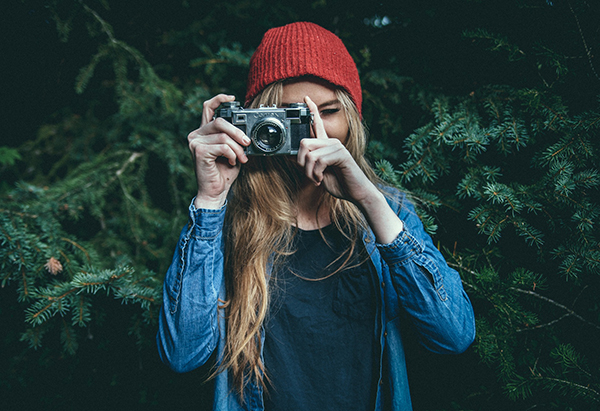
\includegraphics[width=0.8\textwidth]{picture/aa.jpg}
\caption{This giril take a photo.}
\end{figure}

\end{document}